% -*- TeX:UK -*-
\documentclass[10pt]{beamer}
\usetheme{metropolis}
%\useinnertheme{rectangles}
\setbeamercovered{%
still covered={\opaqueness<1->{15}},
again covered={\opaqueness<1->{40}}}

\hypersetup{colorlinks,linkcolor=black,urlcolor=brown,citecolor=brown}

\usepackage{amsmath,amssymb,amsthm}
\usepackage{unicode-math}

% We set the Lucida OTF fonts as default
\usepackage{fontspec}
\setmainfont{Lucida Bright OT}
\setsansfont{Lucida Sans OT}
\setmonofont{Lucida Console DK}[Scale=MatchLowercase]

\newfontfamily\webglyphsfont{WebHostingHub-Glyphs}[Scale=0.7]
\newcommand\webglyphs[1]{{\webglyphsfont\symbol{#1}}}
\newcommand\Discussion{\colorbox{white}{\textcolor{black}{\webglyphs{"F134}}}\xspace}
\newcommand\DiscussionI{\colorbox{black}{\textcolor{white}{\webglyphs{"F134}}}\xspace}
\newcommand\DExamples{\colorbox{black}{\textcolor{white}{\webglyphs{"F134} examples?}}}
\newcommand\Reading{\colorbox{black}{\textcolor{white}{\webglyphs{"F0C1}}}\xspace}
\newcommand\ReadingI{\colorbox{white}{\textcolor{black}{\webglyphs{"F0C1}}}\xspace}
\newcommand\Video{\colorbox{white}{\textcolor{black}{\webglyphs{"F03D}}}\xspace}
\newcommand\Attention{\colorbox{black}{\textcolor{orange}{\webglyphs{"F05A}}}\xspace}
\newcommand\HomeWork{\colorbox{white}{\textcolor{black}{\webglyphs{"F5ED}}}\xspace}
\newcommand\HomeWorkI{\colorbox{black}{\textcolor{white}{\webglyphs{"F5ED}}}\xspace}
\newcommand\Advanced{\colorbox{black}{\textcolor{white}{\webglyphs{"F235}}}\xspace}

\newfontfamily\lineabasicfont{linea-basic-10}
\newcommand\basicicons[1]{{\lineabasicfont\symbol{#1}}}
\newcommand\timeforwards{\basicicons{"0079}}
\newcommand\timebackwards{\basicicons{"0064}}

\newfontfamily\lineaweatherfont{linea-weather-10}
\newcommand\weathericons[1]{{\lineaweatherfont\symbol{#1}}}
\newcommand\meteosun{\weathericons{"E038}}
\newcommand\meteosuncloud{\weathericons{"E042}}
\newcommand\meteorain{\weathericons{"E033}}
\newcommand\meteowind{\weathericons{"E054}}

\newfontfamily\uleaffont{Mini Pics Uprooted Leaf}
\newcommand\uleafmpics[1]{{\uleaffont\symbol{#1}}}
\newcommand\lowplants{\uleafmpics{"00CE}}
\newcommand\mediumplant{\uleafmpics{"006A}}
\newcommand\bush{\uleafmpics{"0039}}
\newcommand\smallplant{\uleafmpics{"0030}}
\newcommand\seedling{\uleafmpics{"002F}}
\newcommand\floweringplant{\uleafmpics{"00CA}}

\newfontfamily\utwigfont{Mini Pics Uprooted Twig}
\newcommand\utwigmpics[1]{{\utwigfont\symbol{#1}}}
\newcommand\grassplant{\utwigmpics{"0033}}

\newfontfamily\uinsectfont{Insect Icons}
\newcommand\uinsect[1]{{\uinsectfont\symbol{#1}}}
\newcommand\bug{\uinsect{"006F}}

\usepackage{polyglossia}
\setdefaultlanguage[variant = british, ordinalmonthday = false]{english}

\usepackage[style=authoryear-comp,firstinits,sortcites,maxcitenames=2,%
    mincitenames=1,maxbibnames=10,minbibnames=10,uniquename=mininit,%
    uniquelist=minyear,sortfirstinits=true]{biblatex}
\addbibresource{../references/ecophys.bib}
\renewcommand{\bibfont}{\small}

\usepackage{abbrev}



\usepackage{tikz}
\usetikzlibrary{positioning,fit,arrows}

\tikzset{
 big dot/.style
  = {circle, draw, inner sep=0pt, minimum size=3mm, fill=teal!50},
 a/.style
  = {node distance=4em, text width=0.1em, minimum height=4em},
 b/.style
  = {rectangle, draw, fill=gray!10, node distance=4em, text width=6em,
     text centered, rounded corners, minimum height=4em, thick},
 c/.style
  = {circle, draw, dashed, fill=orange!10, inner sep = 0pt, node distance=5em, text width=6em,
     text centered, thick},
 d/.style
  = {rectangle, draw, dashed, fill=red!10, node distance=4em, text width=6em,
     text centered, rounded corners, minimum height=4em, thick},
 l/.style
  = {draw, -latex, ultra thick},
 lr/.style
  = {draw, latex-latex, ultra thick, red},
 lb/.style
  = {draw, -latex, ultra thick, blue},
  lo/.style
  = {draw, -latex, ultra thick, orange},
  lg/.style
  = {draw, -latex, ultra thick, teal},
  mylabel/.style
  ={text width=6.5em, text centered},
 aa/.style
  = {node distance=4em, text width=0em, minimum height=0.5ex},
 ll/.style
  = {draw, {open triangle 45} -, thick},
 llb/.style
  = {draw, - triangle 45, thick, blue},
 llg/.style
  = {draw, - open triangle 45, thick, green},
  llt/.style
  = {draw, - open triangle 45, thick, teal},
 llr/.style
  = {draw, - triangle 45, thick, purple},
 llo/.style
  = {draw, - triangle 45, thick, orange}
}

\begin{document}

\title{PBIO-141\\Sensory and Physiological Ecology\\ of  Plants}
\subtitle{3: Signals, cues, information and evolution}
\author{Pedro J. Aphalo}
\date{January-February 2018}
\institute[Univ.\ of Helsinki]{M.Sc.\ in Plant Biology, University of Helsinki\\[2ex] \url{http://blogs.helsinki.fi/aphalo/}}


  \begin{frame}
    \maketitle
  \end{frame}

  \begin{frame}[c]
    \begin{center}
      \begin{small}
        \copyright 2006--2022 by Pedro J. Aphalo\\
        University of Helsinki, Finland.\\
        \textcolor{blue}{\url{http://blogs.helsinki.fi/senpep-blog/}}\\[2ex]
      \end{small}

      \begin{footnotesize}
        Sensory and Physiological Ecology of Plants slides by Pedro J. Aphalo are licensed under a Creative Commons Attribution-ShareAlike 4.0 International License.

      
\includegraphics[width=6em]{../figures/copyright/by-sa}\\[2ex]
      \end{footnotesize}
        
        \begin{scriptsize}
        Typeset in Lucida Sans, \textrm{Luicda Bright}, \texttt{Lucida Console} and Lucida Math. Icons from fonts ``WebHostingHub Glyphs'' (under SIL-Open Font License) from \url{https://www.webhostinghub.com/}; ``insect icons'' (free from \url{http://www.woodcutter.es/}); ``linea-basic-10'' and ``linea-weather-10'' (free from \url{https://github.com/linea-io}), ``Mini Pics Uprooted Twig'' and ``Mini Pics Uprooted Twig'' (commercial, from Image Club Graphics, Inc.). Plant icon as .svg by Abdul Wahhab (free from \url{NounProject.com}).

        Illustrations and text quoted from copyrighted sources is excluded from this license and their use should respect the original licenses.
        \end{scriptsize}
    \end{center}
  \end{frame}


  \begin{frame}
    \frametitle{Outline}
    \tableofcontents
  \end{frame}


\section{The environment and fitness}

\begin{frame}{Cues, Signals and information}{Definitions}
I will use the following set of definitions, although different ones are used by some authors and in other related disciplines.
  \begin{description}
     \item[cue] Stimuli and information originating from inanimate objects, or from organisms for which being a source of information provides \emph{no} `advantage' in fitness.
     \item[signal] Stimuli and information emitted by organisms for which being a source of information provides an `advantage' in fitness.
     \item[communication] Transfer of information between organisms in situations where emission of information is plastic. The transfer of information can be uni- or bidirectional.
     \item[information] Is that which informs, as well as that from which knowledge can be derived.
  \end{description}
\end{frame}

\begin{frame}
  \frametitle{Acclimation: Definitions}
  \begin{description}
    \item[Acclimation, acclimatization] Adjustment by an organism to gradual change in its environment, always within its lifetime.
    \item[Concurrent acclimation] The adjustment to tolerate/profit-from a change in a variable is triggered by the same change event in the same variable.
    \item[Preemptive acclimation] The adjustment to tolerate/profit-from a change in a variable is triggered by the change in other variable(s) which provide an `early warning' of a future environmental condition.
    \item[``Learning''] The adjustment to tolerate/profit-from a change in a variable is triggered by an earlier exposure to a similar change in the same variable.
  \end{description}
\end{frame}

\begin{frame}
\frametitle{Cues, Signals and information \Discussion}
\begin{block}{A plant in a maize field \Discussion 10 + 5 min}
  \begin{itemize}
    \item What cues and signals could a plant use to predict the future?
    \item What information could the plant extract from these cues and signals?
    \item What `decisions' could a plant make based on this information?
    \item Would such decisions affect its success?
    \item Developmental decisions (timing) and acclimation (function and structure) are based on information (from environmental and metabolic signals).
   \end{itemize}
  \end{block}
\end{frame}

\begin{frame}
  \frametitle{The time course of acclimation}

\footnotesize
\resizebox{\linewidth}{!}{%
  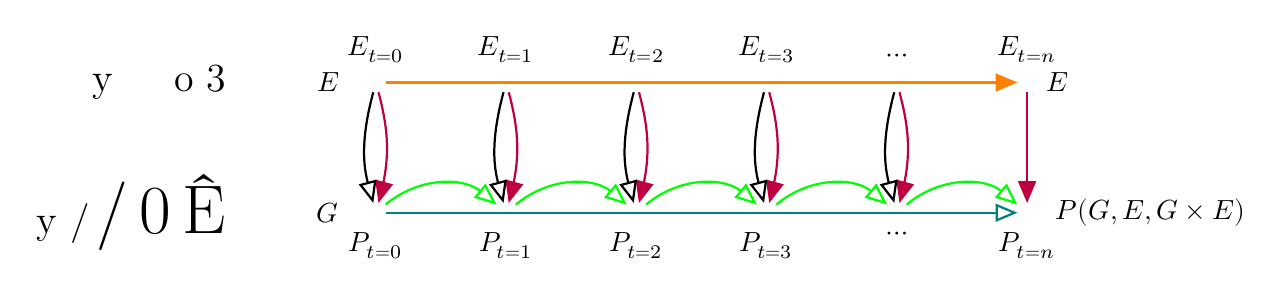
\begin{tikzpicture}[auto]
    \node [aa, label=left:{\Large\timeforwards~\meteosuncloud~\meteorain~\bug~\grassplant}] (environment) {};
    \node [aa, below = of environment, label=left:{\Large\timeforwards~\seedling\,\Huge\seedling\,\smallplant\,\floweringplant}] (plant) {};
    \node [aa, right = of environment, label=above:{$E_{t=0}$}, label=left:{$E\ \ $}] (env_zero) {};
    \node [aa, right = of env_zero, label=above:{$E_{t=1}$}] (env_one) {};
    \node [aa, right = of env_one, label=above:{$E_{t=2}$}] (env_two) {};
    \node [aa, right = of env_two, label=above:{$E_{t=3}$}] (env_three) {};
    \node [aa, right = of env_three, label=above:{$\cdots$}] (env_four) {};
    \node [aa, right = of env_four, label=above:{$E_{t=n}$}, label=right:{$E$}] (env_end) {};
    \node [aa, below = of env_zero, label=below:{$P_{t=0}$}, label=left:{$G\ \ $}] (pheno_zero) {};
    \node [aa, below = of env_one, label=below:{$P_{t=1}$}] (pheno_one) {};
    \node [aa, below = of env_two, label=below:{$P_{t=2}$}] (pheno_two) {};
    \node [aa, below = of env_three, label=below:{$P_{t=3}$}] (pheno_three) {};
    \node [aa, below = of env_four, label=below:{$\cdots$}] (pheno_four) {};
    \node [aa, below = of env_end, label=below:{$P_{t=n}$}, label=right:{\ $P(G, E, G \times E)$}] (pheno_end) {};

    \path [llo, below] (env_zero) -- (env_end);
    \path [llt, above] (pheno_zero) -- (pheno_end);

    \path [llr] (env_zero) edge [bend right=-15] (pheno_zero);
    \path [ll] (pheno_zero) edge [bend right=-15] (env_zero);
    \path [llg, above] (pheno_zero) edge [bend right=-40] (pheno_one);

    \path [llr] (env_one) edge [bend right=-15] (pheno_one);
    \path [ll] (pheno_one) edge [bend right=-15] (env_one);
    \path [llg, above] (pheno_one) edge [bend right=-40] (pheno_two);

    \path [llr] (env_two) edge [bend right=-15] (pheno_two);
    \path [ll] (pheno_two) edge [bend right=-15] (env_two);
    \path [llg, above] (pheno_two) edge [bend right=-40] (pheno_three);

    \path [llr] (env_three) edge [bend right=-15] (pheno_three);
    \path [ll] (pheno_three) edge [bend right=-15] (env_three);
    \path [llg, above] (pheno_three) edge [bend right=-40] (pheno_four);

    \path [llr] (env_four) edge [bend right=-15] (pheno_four);
    \path [ll] (pheno_four) edge [bend right=-15] (env_four);
    \path [llg, above] (pheno_four) edge [bend right=-40] (pheno_end);

    \path [llr] (env_end) -- (pheno_end);

  \end{tikzpicture}%
}%

\textrm{\textbf{Figure:} Time course of one realization of the environment ($E$) during the lifetime of an individual of a genotype ($G$) resulting in a phenotype ($P$).}

\end{frame}

\begin{frame}
  \frametitle{Preemptive acclimation: A simple model}

\footnotesize
\resizebox{\linewidth}{!}{%
  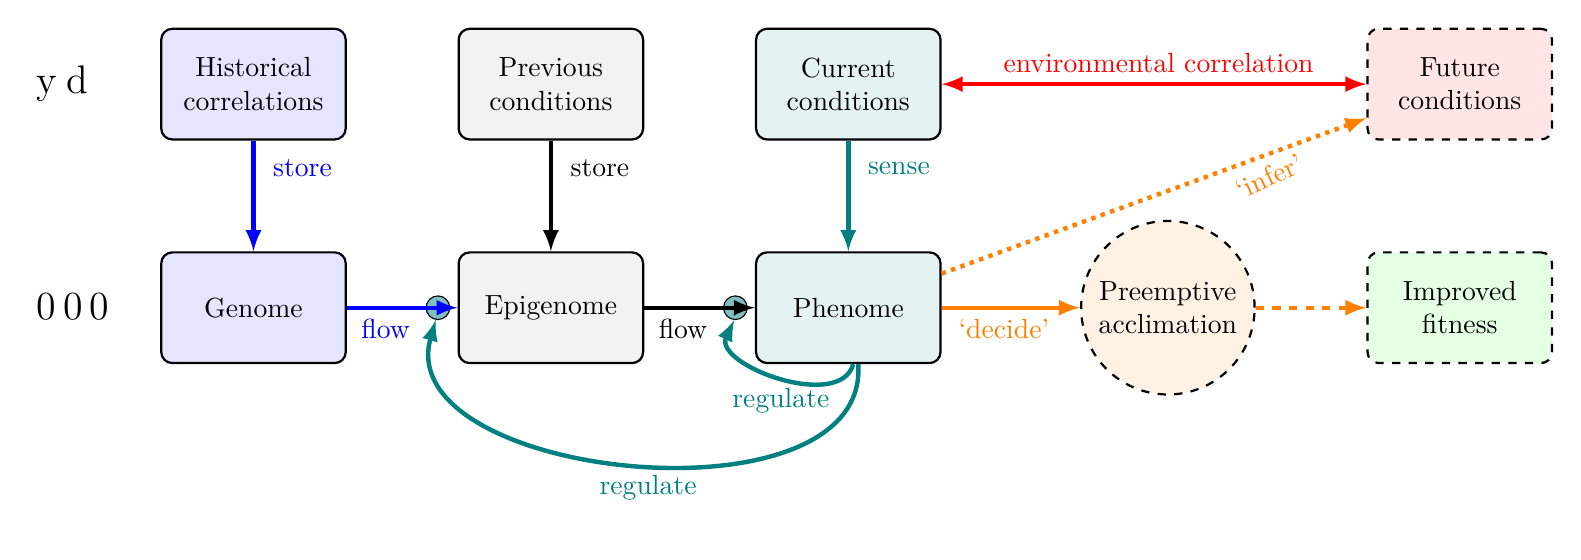
\begin{tikzpicture}[auto]
    \node [a] (environment) {\Large\timeforwards~\timebackwards};
    \node [b, right = of environment, fill=blue!10] (history) {Historical correlations};
    \node [b, right = of history] (stress) {Previous conditions};
    \node [b, right = of stress, fill=teal!10] (data) {Current conditions};
    \node [b, below = of history, fill=blue!10] (genome) {Genome};
    \node [big dot, right = of genome] (valve1) {};
    \node [b, below = of stress] (memory) {Epigenome};
    \node [big dot, right = of memory] (valve2) {};
    \node [b, right = of memory, fill=teal!10] (info) {Phenome};
    \node [a, below = of environment] (plant) {\Large\smallplant\,\smallplant\,\smallplant};
    \node [c, right = of info, fill=orange!10] (acclimation) {Preemptive acclimation};
    \node [d, right = of acclimation, fill=green!10] (ready) {Improved fitness};
    \node [d, above = of ready] (stress2) {Future conditions};

    \path [l] (stress) -- (memory) node[near start,right]{\hspace{0.3em}store};
    \path [lb] (history) -- (genome) node[near start, right]{\hspace{0.3em}store};
    \path [lg] (data) -- (info) node[near start,right]{\hspace{0.3em}sense};
    \path [lb] (genome) -- (memory) node[near start,below]{\hspace{0.8em}flow};
    \path [l] (memory) -- (info) node[near start,below]{\hspace{0.8em}flow};
    \path [lr] (stress2) -- (data) node[near end,above]{\hspace{8em}environmental correlation};
    \path [lo, dotted] (info) -- (stress2) node[near end,below,rotate=25]{`infer'};
    \path [lo] (info) -- (acclimation) node[near start,below]{\hspace{2em}`decide'};
    \path [lo, dashed] (acclimation) -- (ready);
    \path [lg] (info) edge [bend left=100]  node[midway, below]{\hspace{1em}regulate} (valve1);
    \path [lg] (info) edge [bend left=95]  node[midway, below]{regulate\hspace{5em}} (valve2);

\end{tikzpicture}%
}%


{\tiny Flow of information in preemptive acclimation. Arrows represent flows of information: \textcolor{blue}{\textbf{blue}} = retrieved from genome (stored during evolution), \textbf{black} = acquired during an individual's or its progenitor's lifetime, \textcolor{teal}{\textbf{teal}} = regulation of gene expression by phenome or downward causation, \textcolor{red}{\textbf{red}} = lagged correlation between two or more environmental variables, \textcolor{orange}{\textbf{orange}} = outcome of information processing, which is a developmental ‘decision’ based on an implicit environmental forecast and with implications for fitness. \textcolor{green}{\textbf{green}} = future phenotype with `improved fitness' relative, in probabilistic terms, to no acclimation. Dashed boxes and arrows represent the likely or forecasted future. Conditions refer to cues and signals both in the environment and plant's internal status, corresponding to phenotypic plasticity, and developmental plasticity respectively.}

\end{frame}

\begin{frame}{Acclimation and developmental plasticity}
\textbf{Problem-solving or decision-making perspective}
    \begin{itemize}
      \item What problems does a plant need to solve through its lifetime?
      \item Discussion
      \item Some examples:
        \begin{itemize}
          \item Timing and place of germination.
          \item How to reach the soil surface.
          \item When to start producing chlorophyll.
          \item How tall to grow.
          \item In which direction to grow (both above- and belowground).
          \item Where to position the leaves and roots.
          \item How to protect from enemies.
          \item When to emit signals and which ones.
          \item When to flower.
        \end{itemize}
    \end{itemize}
\end{frame}

\begin{frame}
  \frametitle{Environmental correlations and forecasting \Discussion}
  \begin{itemize}
    \item Correlations in the environment of a plant
    \item What information do they carry?
    \item Can you think examples of their use by plants?
    \item Can organisms `generate' environmental correlations to their benefit?
    \item Do organisms cheat? Provide false information to deceive other organisms?
  \end{itemize}
\end{frame}

\section{Memory, communication, and intelligence}

\begin{frame}{What is memory?}
\begin{itemize}
  \item Memory is storage of information in a way that can be recalled
  \item Long-term `memory' in organisms is the genome
  \item Medium-term `memory' is mostly in the epigenome
  \item Shortest-term `memory' is in cell signalling and metabolic regulation
  \item This is a useful oversimplification, so be careful!
  \item The world cannot be described in three shades of grey...
\end{itemize}
\end{frame}

\begin{frame}
\frametitle{Plants store information}
  \begin{itemize}
    \item It has been shown that plants can `remember' past experiences.
    \item For example the experience of cold is remembered (this is called vernalization).
    \item There is also evidence that seeds of equal genotype, but that have formed under different environmental conditions, can produce plants with different phenology.
    \item There is also some recent evidence of trans-generational memory, by which the environment under which parents have grown affects the behaviour of siblings.
%    \item The capacity of plants to remember is dependent in many cases on epigenetic gene regulation, but other mechanisms like accumulation of metabolite precursors, or receptor proteins has also been suggested.
  \end{itemize}
\end{frame}

\begin{frame}
\frametitle{Communication within the plant}
  \begin{itemize}
    \item There is communication within plants.
    \item The responses of different parts of an individual plant are coordinated.
    \item This is not just a question of resource partition.
    \item In plants there are hormones, small proteins, miRNAs, likely even electrical signals, moving from one place to another and transferring information.
    \item For example a short time after irradiation of the shoot of a maize plant with ultraviolet radiation, gene expression changes both in the shoots and roots of the plant, and regulated genes are not all the same ones in both parts.
    \item Soil drying is sensed by roots and plant hormones transfer this information to leaves (and leads to adjustment of stomatal opening).
  \end{itemize}
\end{frame}

\begin{frame}
\frametitle{Communication outwith the plant I}
  \begin{itemize}
    \item There is communication between plants.
    \item The responses of different plants are to some extent coordinated.
    \item This is not just a question of resource depletion.
    \item Plants change the light environment (most likely a cue) allowing the detection of neighbours before competition for light starts.
    \item Plants can recognize their own roots as different from those of neighbours and use this information to adjust behaviour.
  \end{itemize}
\end{frame}

\begin{frame}
\frametitle{Communication outwith the plant II}
  \begin{itemize}
    \item Plants emit volatile metabolites that work as `alarm signals', informing other plants and other parts of the same plant, of for example impending attack by herbivore insects.
    \item Plants emit volatile metabolites that work as `alarm signals', informing the predators of the herbivores that there are insects to be eaten.
    \item It has been proposed that plants being eaten by herbivore insects can produce UV-absorbing pigments that `tag' the attacked leaves making them easier for predator birds to find.
  \end{itemize}
\end{frame}

\begin{frame}
\frametitle{Communication outwith the plant III}
  \begin{itemize}
    \item There is current research on signaling between roots through the soil: for example closure of stomata in unstressed plants when they partially share the rooting space with salt stressed plants. The phenomenon has been demonstrated, but the mechanism is still under investigation, but release of the plant hormone ABA seems to be involved.
    \item Research on the synchronization of other responses like flowering has shown that communication through roots is used.
    \item I am not yet aware of research on the fitness advantages of synchronization, but one can imagine advantages at the population level\ldots
    \item \ldots on the other hand there are analyses explaining how altruism could have evolved, for example in birds and even in bacteria.
\end{itemize}
\end{frame}

\begin{frame}
\frametitle{Are plants intelligent? \Discussion 5 min}
    \begin{itemize}
        \item This is very controversial.
        \item As proposed by \citetitle{Trewavas2014} \autocite{Trewavas2014}, plants could be considered intelligent with a similar definition of intelligence as used for `artificial intelligence' in computer science.
        \item If they are intelligent, they have a very different implementation of the problem solving capacity.
        \item If one stretches the definition far enough, I think one could consider every living organism as intelligent.
        \item But is it necessary to use the word `intelligent' for plants and bacteria? Does it help understanding or makes it more difficult?\\[1ex]
        \emph{\textbf{What do you think?}} (5 min)
    \end{itemize}
\end{frame}

\section{A new paradigm}

\begin{frame}
\frametitle{A new paradigm is emerging}
\textbf{An exciting time to study plants!!}
    \begin{itemize}
      \item Currently it is a very exciting time to study plants\ldots
      \item \ldots especially how their molecular biology, evolution and ecology are linked.
      \item We are in the middle of a paradigm shift\ldots
      \item \ldots for a long time we have disregarded the sensory and problem-solving abilities of plants.
      \item However, we should be open minded and use our imagination to understand plant life as it is\ldots
      \item \ldots rather than to project `human' features and qualities onto plants.
    \end{itemize}
\end{frame}

\begin{frame}
  \frametitle{Preemptive acclimation: What is the evidence?}
  \begin{itemize}
    \item Several plant responses can be only explained from the evolutive/fitness
    point of view as being a `preparation' to tolerate or escape future stress events or
    take advantage of future favourable conditions.
    \item Preemptive shade avoidance as a response to reflected far-red light from neighbouring
    plants.
    \item Possibly (a hypothesis we are studying) preemptive acclimation to future soil
    drying in response to high ultraviolet-B irradiance.
    \item Eavesdropping-on/communicating-with neighbours to preemptively acclimate/prepare
    for drought, herbivore attacks, even to synchronize flowering among individuals.
  \end{itemize}
\end{frame}

\begin{frame}
  \frametitle{Self vs.\ alien recognition: What is the evidence?}
  \begin{itemize}
    \item Roots in the soil grow differently when near another root of the same plant than
    when near roots of a different plant (even if the two plants have the same genotype).
    \item There is keen recognition by shoots dependent on light perception (plants respond
    differently depending on the species of the neighbours).
  \end{itemize}
\end{frame}

\section{General discussion}

\begin{frame}
\frametitle{Environmental correlations and forecasting \Discussion}

\textbf{Can plants `predict' the arrival of the cold season?\\
 What sources of information do they use?}

    \centering
    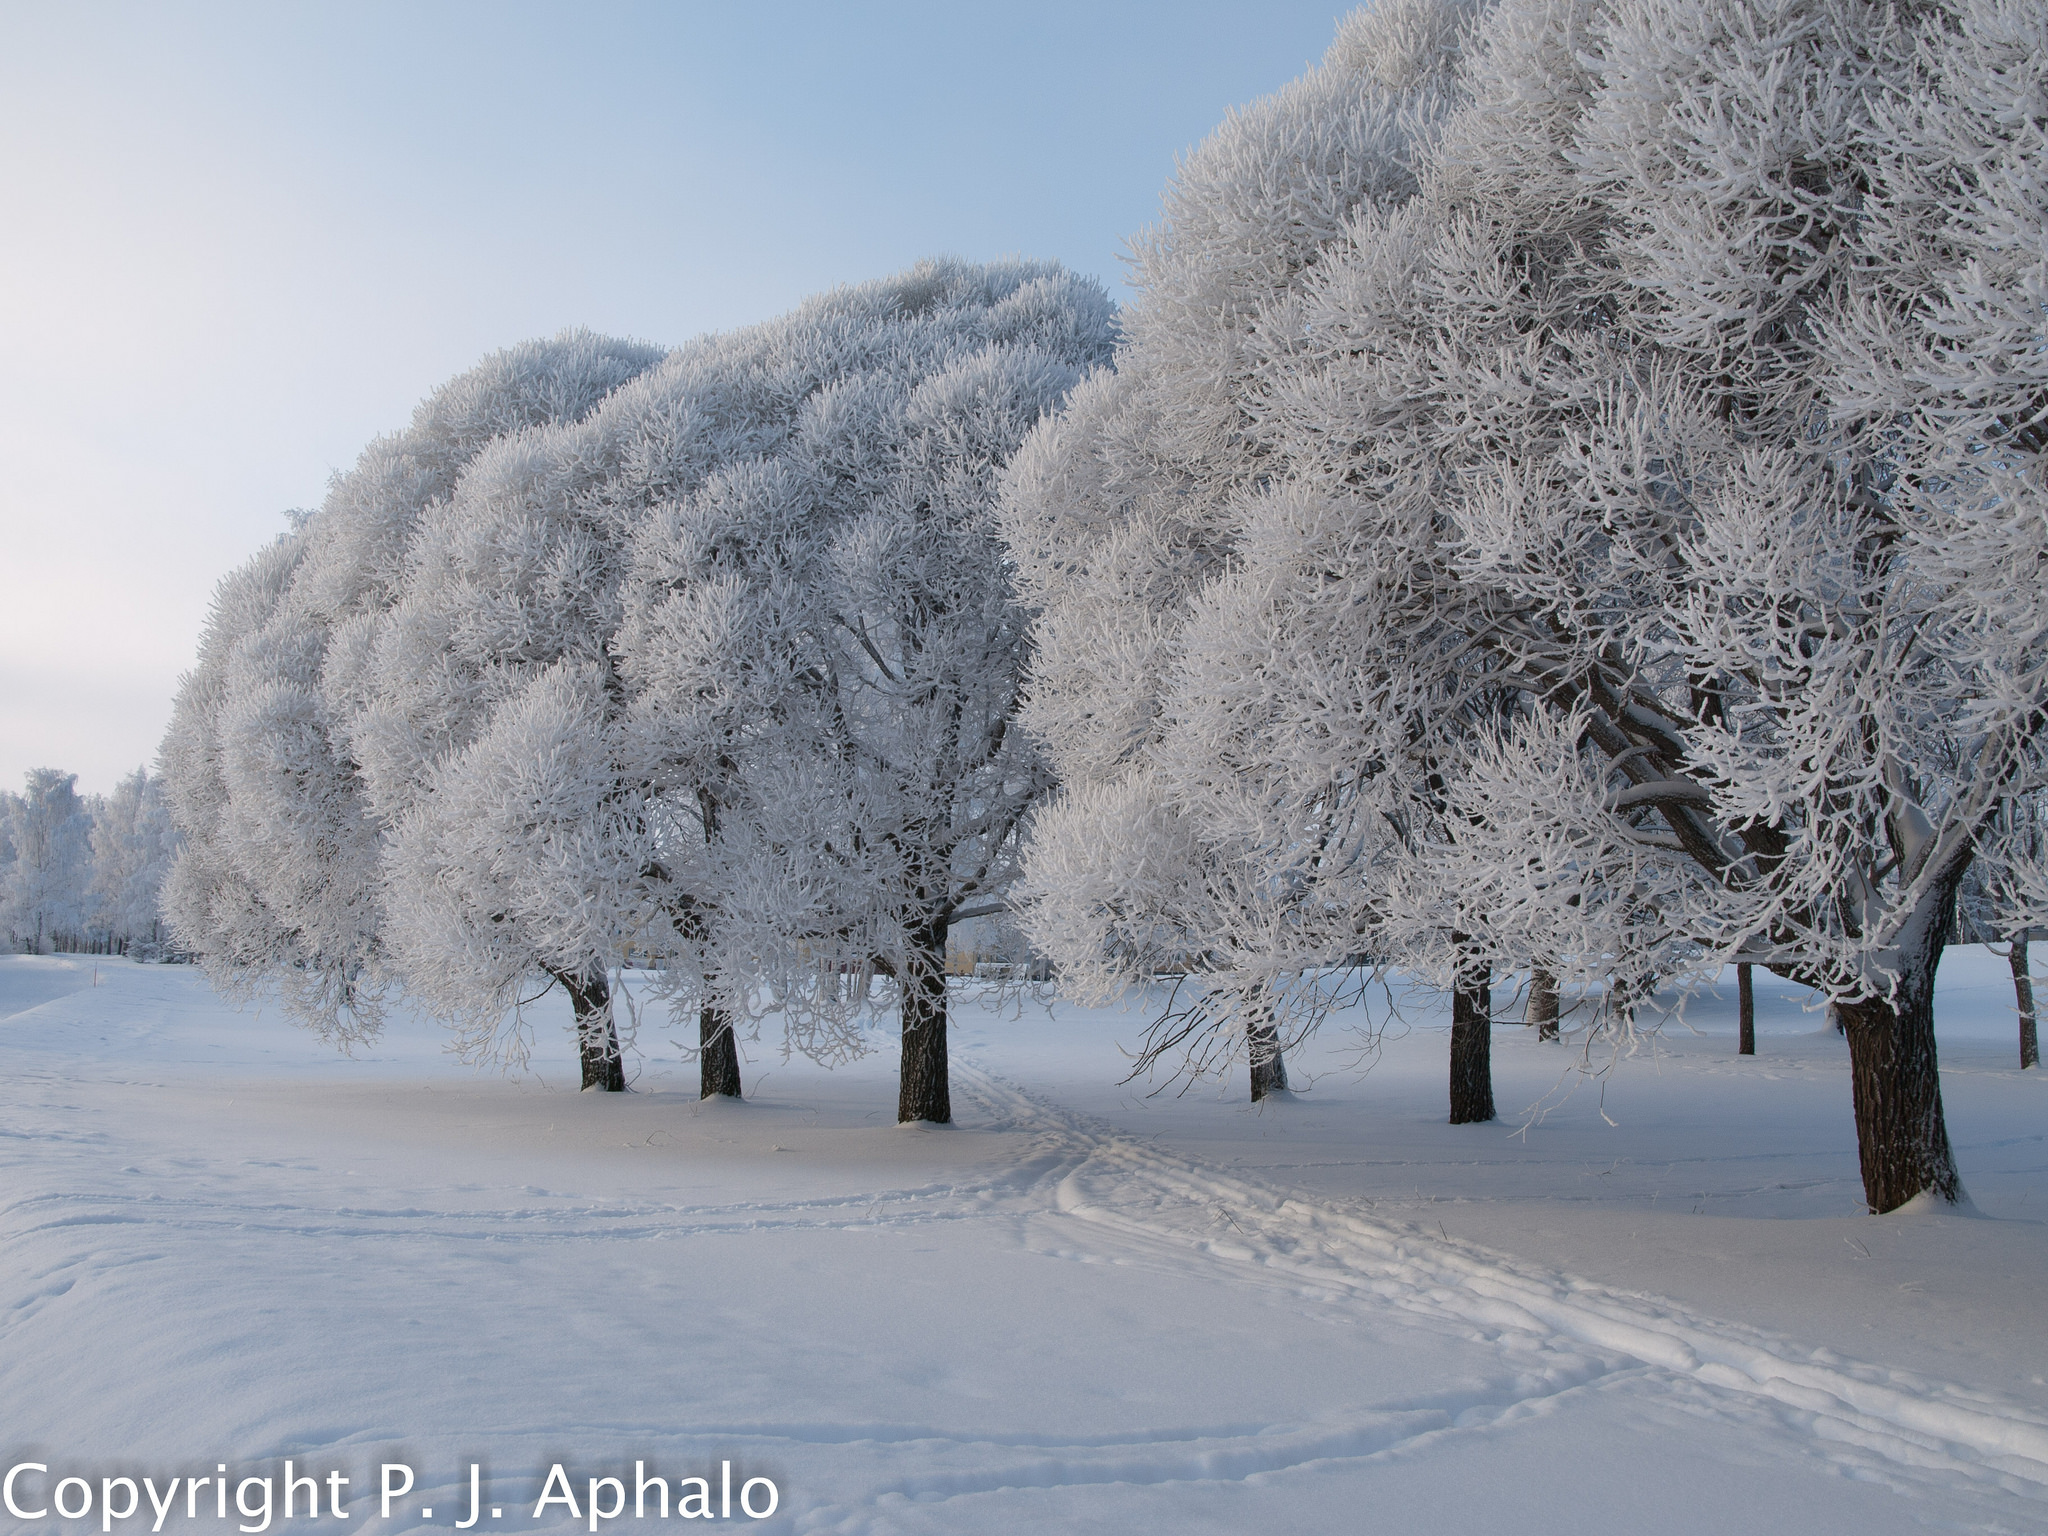
\includegraphics[height=0.75\textheight]{../photos/winter}
\end{frame}

\begin{frame}
\frametitle{Environmental correlations and forecasting \Discussion}

\textbf{Can plants `predict' the arrival of the spring?\\
 What sources of information do they use?}

    \centering
    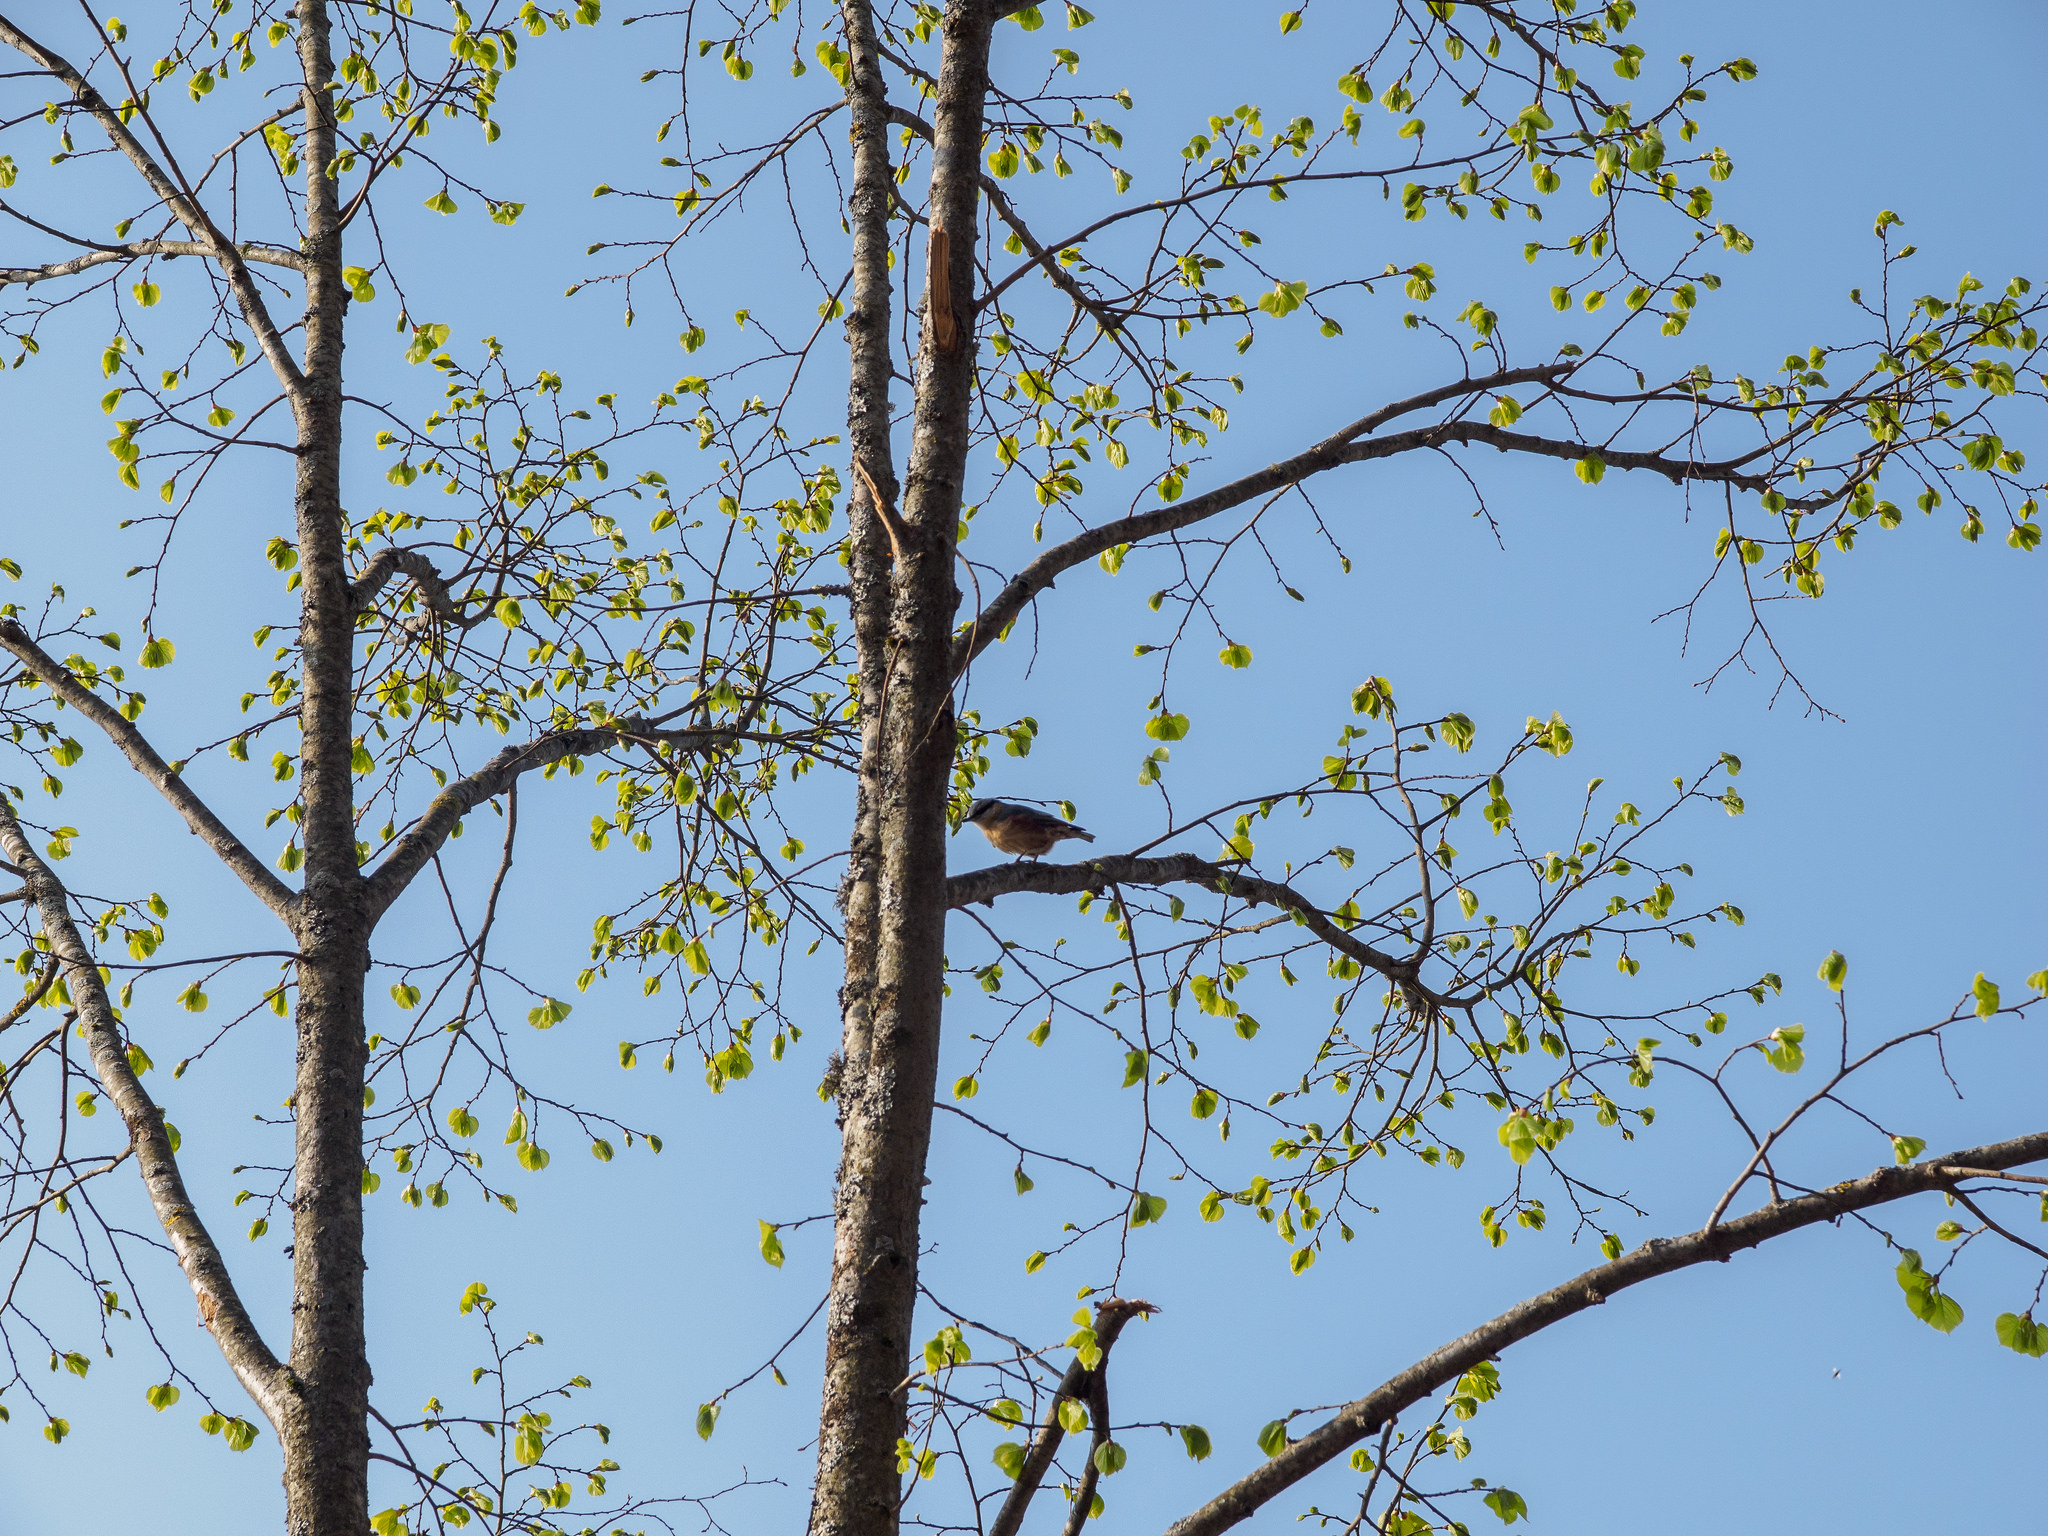
\includegraphics[height=0.75\textheight]{../photos/spring}
\end{frame}

\begin{frame}
\frametitle{Environmental correlations and forecasting \Discussion}

\textbf{Can plants emit `signals' for their benefit?\\
What are the signals used to attract pollinators?}

    \centering
    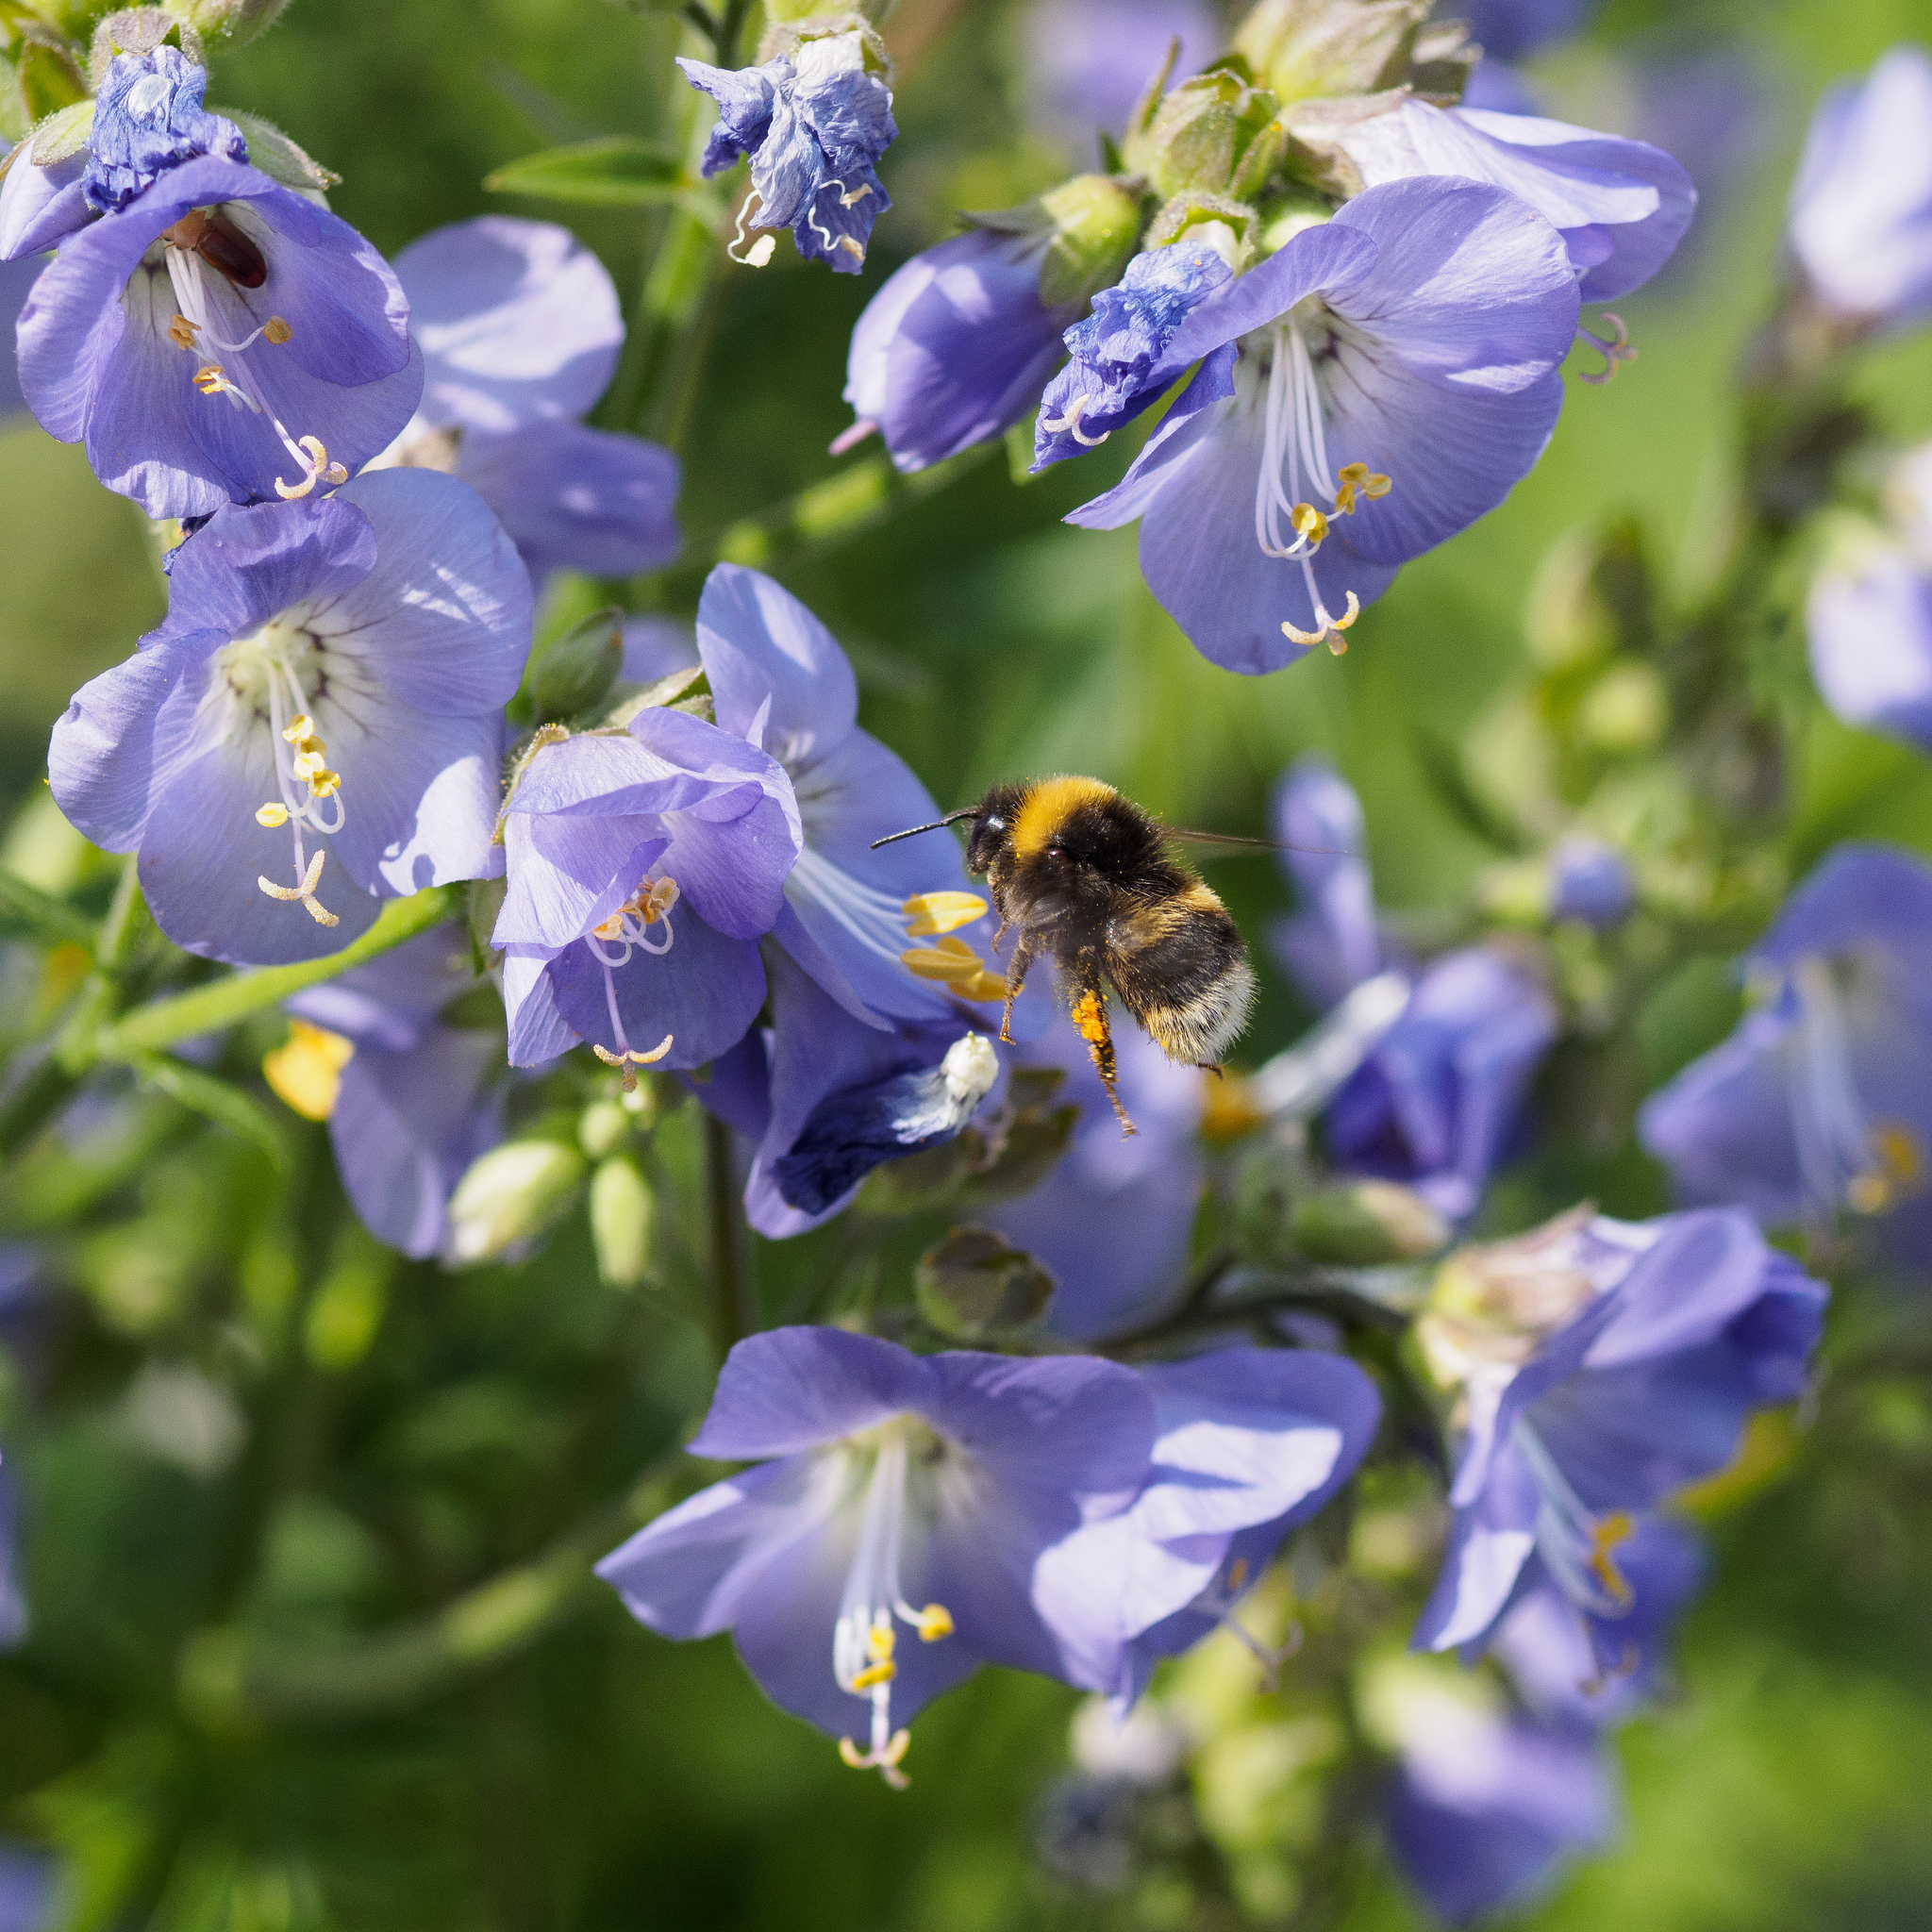
\includegraphics[height=0.75\textheight]{../photos/bumblebee}
\end{frame}

\begin{frame}
\frametitle{Environmental correlations and forecasting \Discussion}

\textbf{Can plants emit `signals' for their benefit?\\
What are the signals used to enlist ``helpers'' for seed dispersal?}

    \centering
    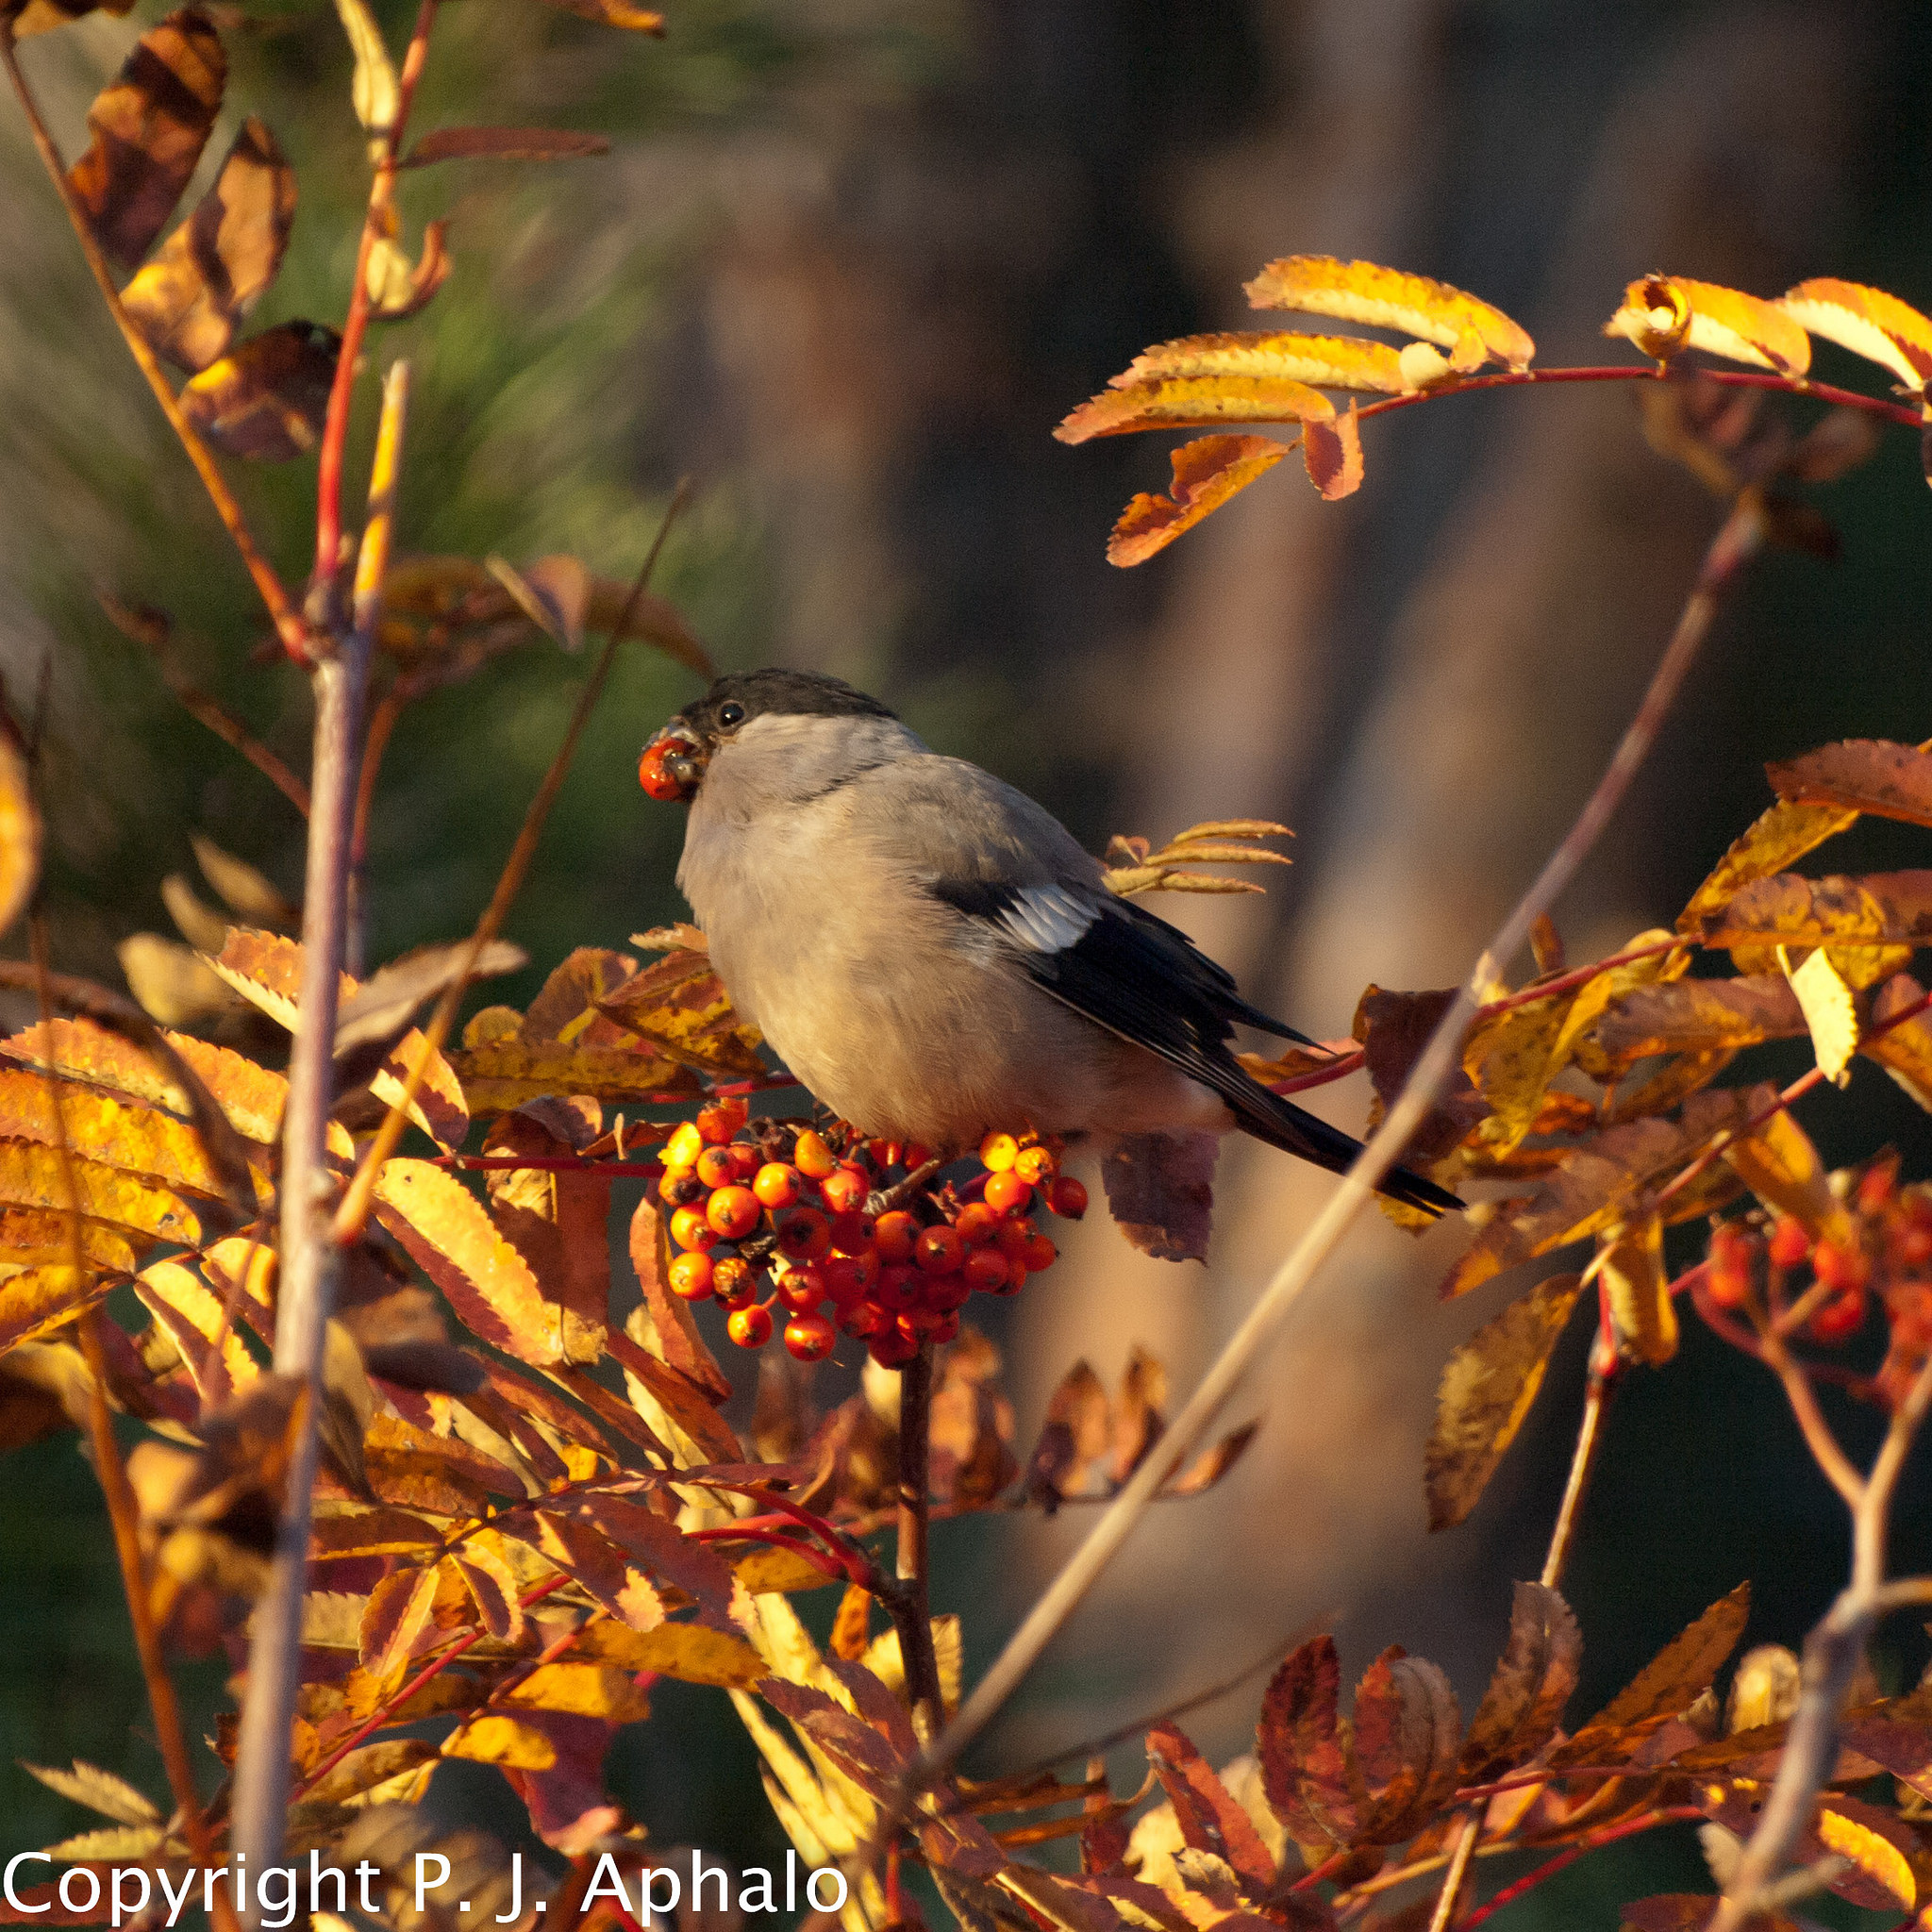
\includegraphics[height=0.75\textheight]{../photos/berry_eater}
\end{frame}

\begin{frame}
\frametitle{Environmental correlations and forecasting \Discussion}

\textbf{Can plants emit signals to deceive other organisms?\\
How does mimicry work?}

    \centering
    \includegraphics[height=0.75\textheight]{../photos/nettle}
\end{frame}

\begin{frame}
\frametitle{Environmental correlations and forecasting \Discussion}

\textbf{Can plants `generate' environmental correlations for their benefit?\\
How does release of organic volatile compounds create a correlation?}

    \centering
    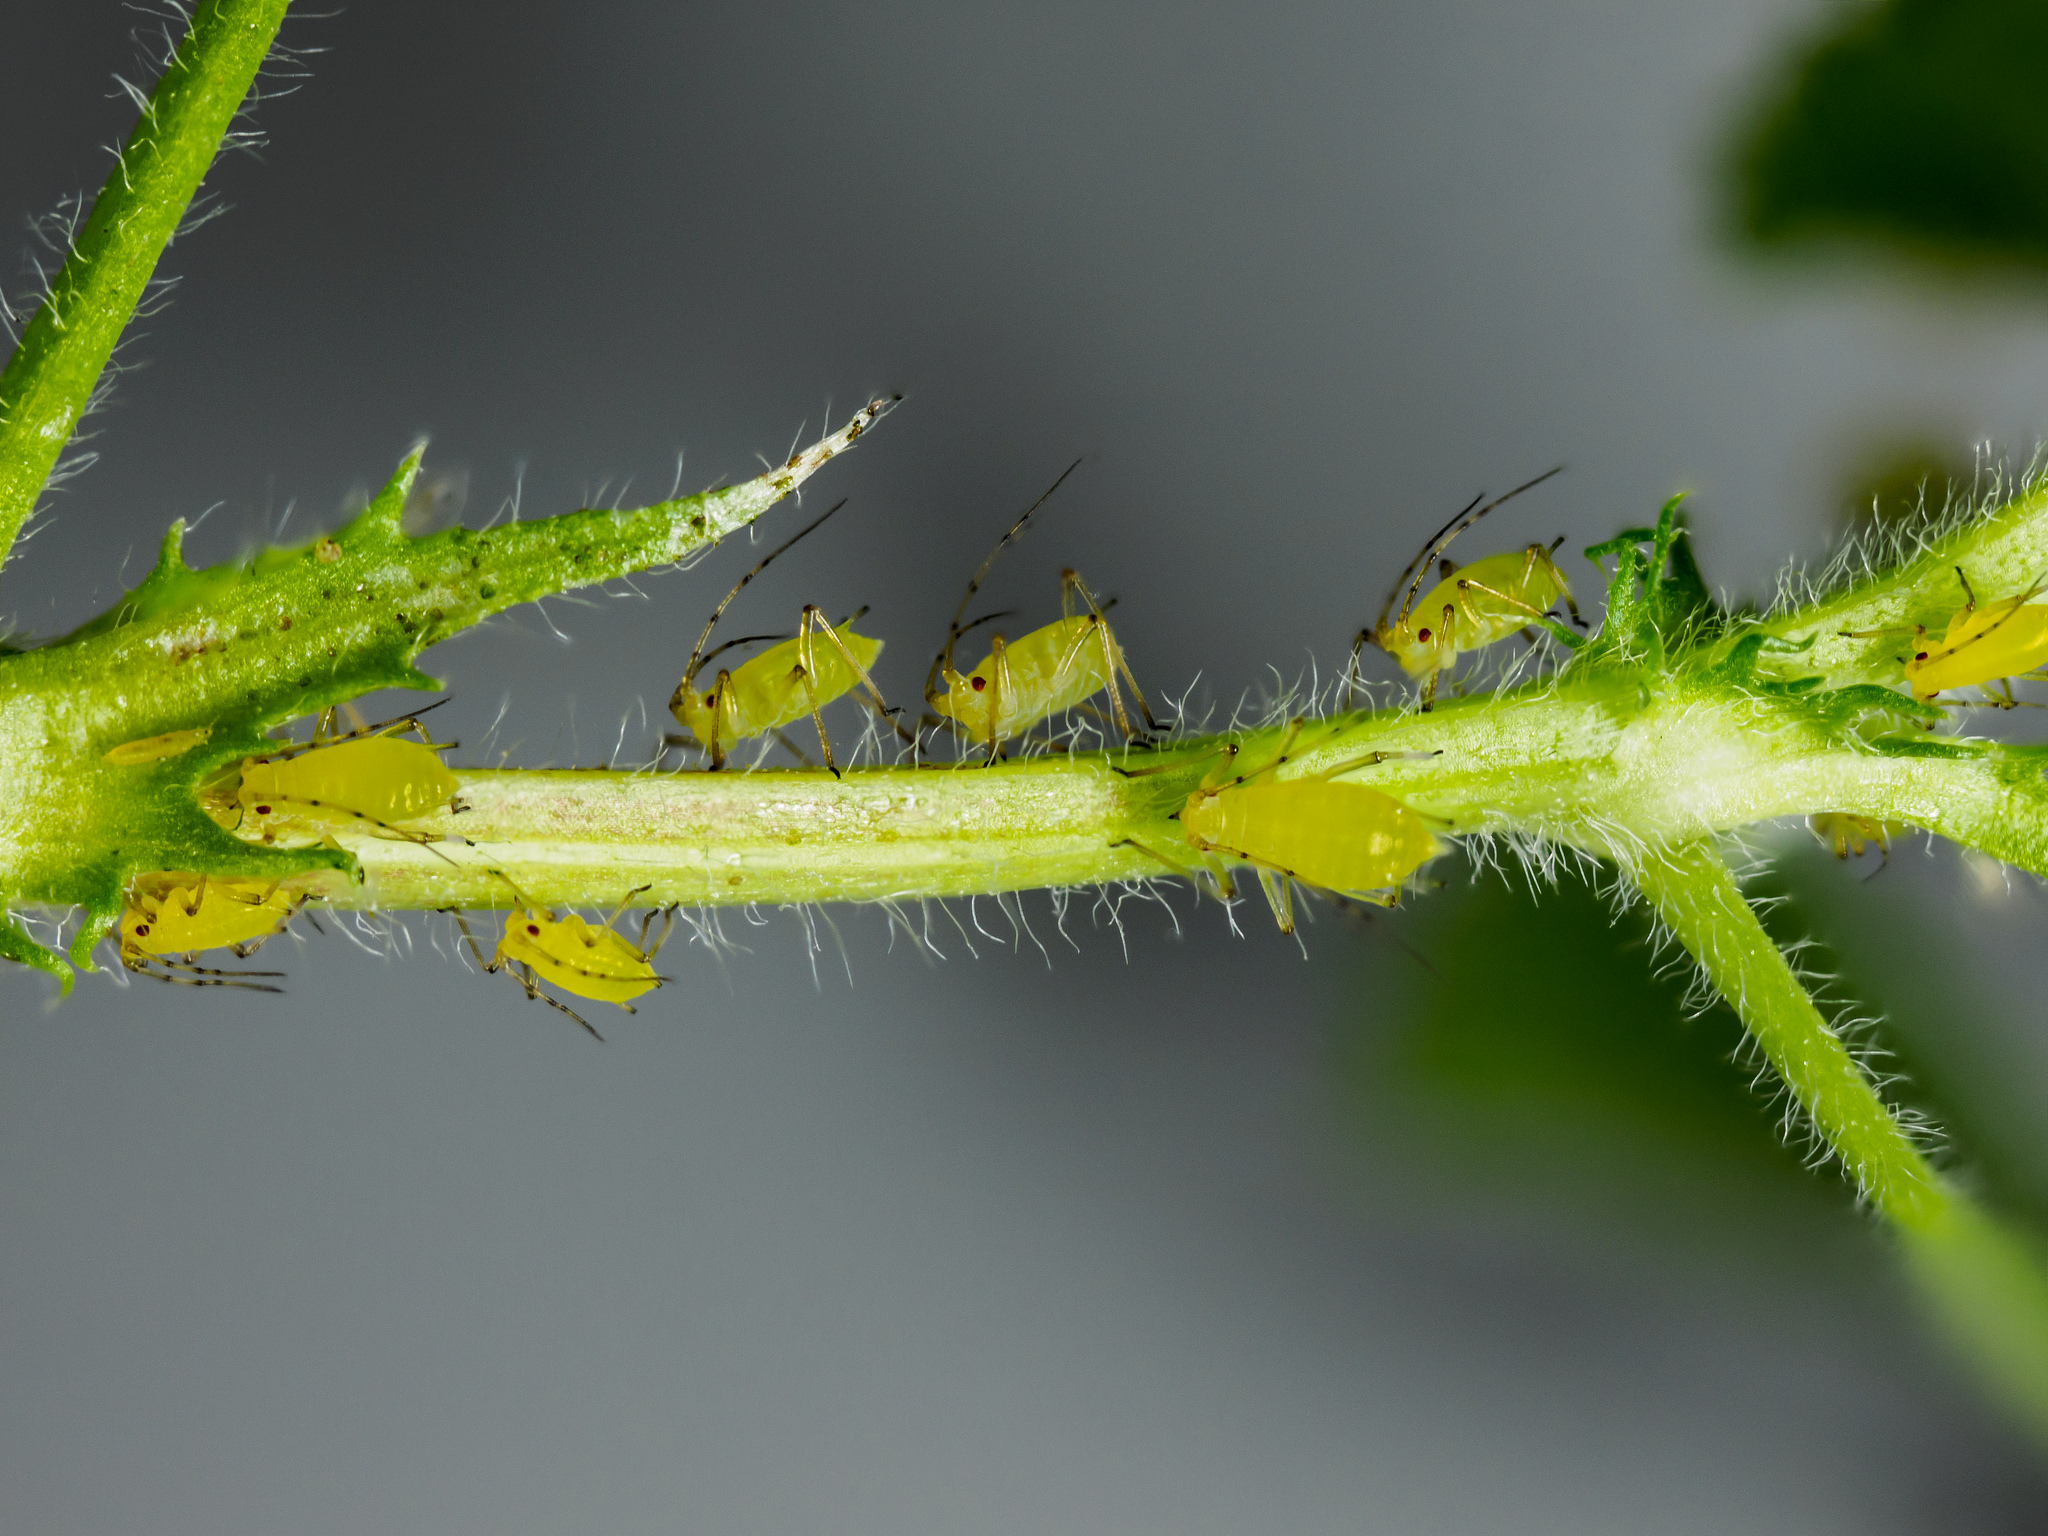
\includegraphics[height=0.7\textheight]{../photos/aphids}
\end{frame}

\begin{frame}
\frametitle{Symbioses: ectomycorrhizas \Discussion}

\textbf{Do symbioses involve communication?}

    \centering
    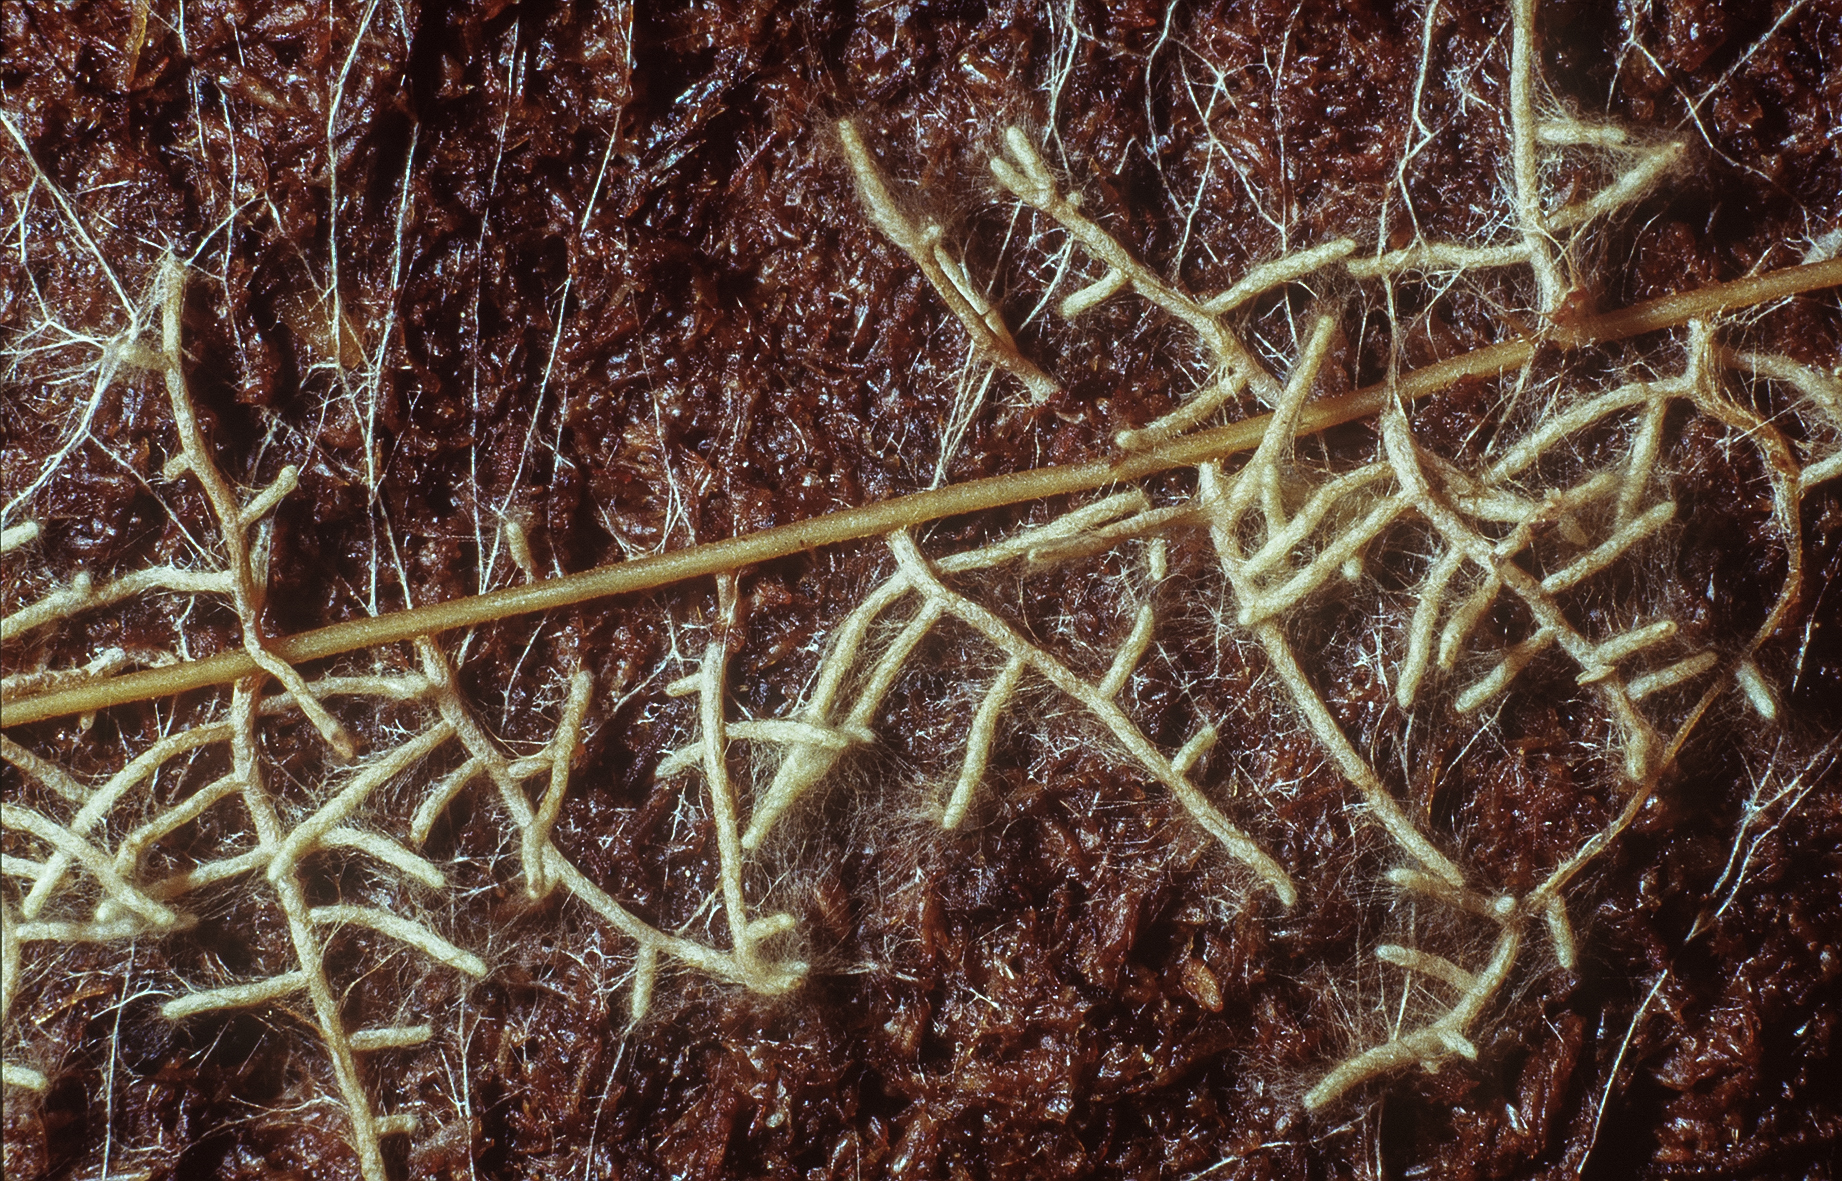
\includegraphics[height=0.75\textheight]{../photos/dia3}
\end{frame}



%\begin{frame}{Discussion}{One question per pair of students (10 min), whole class (10 min)}
%  After listening to this lecture, what would you think if someone told you that:
%  \begin{itemize}
%    \item plants display behaviour?
%    \item plants can learn?
%    \item plants can perceive their environment?
%    \item plants can solve problems?
%    \item plants have intelligence?
%    \item how does this affect crop breeding and management?
%    \item how could this affect ecosystem response to climate change?
%  \end{itemize}
%\end{frame}

  \section*{References}
  \begin{frame}[t,allowframebreaks]
    \frametitle{References}
    \printbibliography
  \end{frame}

\end{document}
